%%% LaTeX Template: Article/Thesis/etc. with colored headings and special fonts
%%%
%%% Source: http://www.howtotex.com/
%%% Feel free to distribute this template, but please keep to referal to http://www.howtotex.com/ here.
%%% February 2011
%%%
%%% Modified October 2015 by CDM

%%%  Preamble
\documentclass[11pt,letterpaper]{article}
\usepackage[margin=1.0in]{geometry}
\usepackage[T1]{fontenc}
\usepackage[bitstream-charter]{mathdesign}
\usepackage[latin1]{inputenc}					
\usepackage{amsmath}						
\usepackage{xcolor}
\usepackage{cite}
\usepackage{hyphenat}
\usepackage{graphicx}
\usepackage{float}
\usepackage{subfigure}
\usepackage{sectsty}
\usepackage[compact]{titlesec} 
\usepackage[tablegrid]{vhistory}
\usepackage[parfill]{parskip}
\allsectionsfont{\color{accentcolor}\scshape\selectfont}

%%% Definitions
\definecolor{accentcolor}{rgb}{0.0,0.0,0.5} 
\newcommand{\teamname}{Project Iris}
\newcommand{\productname}{Iris}
\newcommand{\coursename}{CSE 4316: Senior Design I}
\newcommand{\semester}{Summer 2016}
\newcommand{\docname}{Project Charter}
\newcommand{\department}{Department of Computer Science \& Engineering}
\newcommand{\university}{The University of Texas at Arlington}
\newcommand{\authors}{Neil Simmons \\ Tyler D'Spain \\ Matthew Zielke \\ Syed Uddin \\ Tony McDonald}

%%% Headers and footers
\usepackage{fancyhdr}
	\pagestyle{fancy}						% Enabling the custom headers/footers
\usepackage{lastpage}	
	% Header (empty)
	\lhead{}
	\chead{}
	\rhead{}
	% Footer
	\lfoot{\footnotesize \teamname \ - \semester}
	\cfoot{}
	\rfoot{\footnotesize page \thepage\ of \pageref{LastPage}}	% "Page 1 of 2"
	\renewcommand{\headrulewidth}{0.0pt}
	\renewcommand{\footrulewidth}{0.4pt}

%%% Change the abstract environment
\usepackage[runin]{abstract}			% runin option for a run-in title
%\setlength\absleftindent{30pt}			% left margin
%\setlength\absrightindent{30pt}		% right margin
\abslabeldelim{\quad}	
\setlength{\abstitleskip}{-10pt}
\renewcommand{\abstractname}{}
\renewcommand{\abstracttextfont}{\color{accentcolor} \small \slshape}	% slanted text

%%% Start of the document
\begin{document}

%%% Cover sheet
{\centering \huge \color{accentcolor} \sc \textbf{\department \\ \university} \par}
\vspace{1 in}
{\centering \huge \color{accentcolor} \sc \textbf{\docname \\ \coursename \\ \semester} \par}
\vspace{0.5 in}
\begin{figure}[h!]
	\centering
   	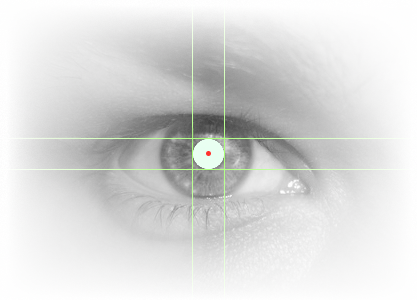
\includegraphics[width=0.60\textwidth]{images/project-iris}
\end{figure}
\vspace{0.5 in}
%%{\centering \huge \color{accentcolor} \sc \textbf{\teamname \\ \productname} \par}
{\centering \huge \color{accentcolor} \sc \textbf{\teamname} \par}
\vspace{0.5 in}
{\centering \large \sc \textbf{\authors} \par}
\newpage


%\vspace{1 in}
%\centerline{January 13th, 2012}
%\newpage

%%% Revision History
\begin{versionhistory}
  	\vhEntry{0.1}{07.09.2016}{NS\textbackslash{}TS\textbackslash{}MZ\textbackslash{}SU\textbackslash{}TM}{document creation}
\end{versionhistory}
\newpage

%%% Table of contents
\tableofcontents
\newpage

%%% List of figures and tables (optional)
\listoffigures
%\listoftables
\newpage

%%% Agile project charter sections
\section{Vision}

In a world of mice and keyboards we believe a PC input peripheral device is missing, and that device is a 3D gaze tracker. The most expressive part of a human's anatomy is their eyes. They can convey surprise, sadness, joy, and love. With the Project Iris we aim to help them add a new dimension to their capabilities, and in turn add new capability to the PC as well. This will not only enable new user experiences for PCs and software developers, but also enable PC experiences for the disabled and handicapped as well. A group that can find it difficult to interact with current PC technology.

The new experiences created may give greater control in a video game by allowing a user to make selections with their eyes, without shifting hands off the keyboard or changing the mouse's focus. We envision our solution enabling artist to visually switch between tools in paint programs by allowing them to look at the tool they wish to use, rather than taking their hand away from their artwork. For a musician, switching backing tracks or audio effects between songs is currently clunky, but we believe by using their vision they can adjust their tools, without taking their hands off their instruments. More importantly we believe that we don't know all the possibilities this software may have, which is why we want it to be open source, to allow others with a vision to expand upon ours.
\section{Mission}

To design an open source 3D gaze tracking software solution using off the shelf, fully integrated hardware. We will design this solution using the Intel RealSense SR300 camera. It combines a traditional 2D video camera and a 3D infrared camera designed to work in the sorter ranges expected with PC use. In addition, the Intel RealSense cameras are already integrated into some laptops, allowing our solution to be more readily adopted. 

We will design the system to operate as a visual mouse, enabling either the user's eyes to act as a pseudo mouse input, or to act as a selection device that leaves the traditional mouse free for normal use. We will accomplish this using the 3D data provided by the RealSense camera in conjunction with its 2D camera data. Mathematical operations will be performed to isolate a user's eyes and track them in relation to the camera that is setting near the screen. Once calibrated the combination of 3D and 2D inputs will allow the software to follow the users gaze, thereby enabling the input functionality of the software. Additional functionality be added for input purposes; blink and wink detection will be added, as well as algorithms to detect eye movement patterns. 

\section{Success Criteria}

For Project Iris to be considered a success it must be complete and working by The end of the 2016 fall semester.  The camera will track the gaze of the eye and a user will have the ability to view the position of their eyes visually on screen.  The project will make available an API where-by developers may integrate eye position data into their projects. The project will also provide a toggle via API calls to enable on-screen display of the current eye position. Additionally a calibration utility and a camera output data visualization utility will be provided.
\newpage

%%% Remaining project charter sections
\section{Background}

Project Iris consists of a diverse group of members.  A Computer Engineer, a Software Engineer, and three Computer Scientists.  This diversity gives the team a great advantage because each member will be able to approach the project from a different view point, using the skills and knowledge gained from each members course work.
\section{Related Work}

For the past couple years gaze tracking has been a hot item for researchers.  Previously, the use of a Microsoft Kinect device was used to impose gaze tracking without the use of a full infrared system.  The team at Microsoft Research published an article relating to gaze tracking using feature detection with a Microsoft Kinect.  However, work related to creating a virtual mouse has been mostly proprietary or expensive in assistive technologies.  Because of the optimal distances that are required for a Kinect,  a virtual pointer has only been effective with the use of algorithms to determine selection.
\section{System Overview}
This section should describe the overall structure of your software system. Think of it as the strategy for how you will build the system. An architectural "layer" is the top-level logical view, or an abstraction, of your design. Layers should be composed of related elements of similar capabilities, and should be highly independent of other layers, but should have very clearly defined interfaces and interactions with other layers. Each layer should be identified individually and should be unique as to its function and purpose within the system. This section should also contain the high-level block diagram of the layers, as shown in the example below, as well as detailed descriptions of the functions of each layer.

\begin{figure}[h!]
	\centering
 	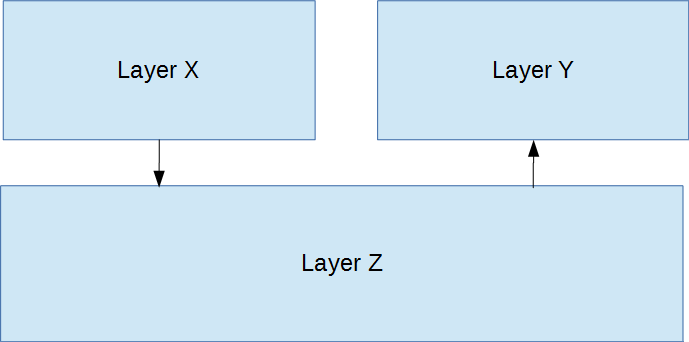
\includegraphics[width=0.60\textwidth]{images/layers}
 \caption{A simple architectural layer diagram}
\end{figure}

\subsection{Layer X Description}
Each layer should be described separately in detail. Descriptions should include the features, functions, critical interfaces and interactions of the layer. The description should clearly define the services that the layer provides. Also include any conventions that your team will use in describing the structure: naming conventions for layers, subsystems, modules, and data flows; interface specifications; how layers and subsystems are defined; etc. 

\subsection{Layer Y Description}
Each layer should be described separately in detail. Descriptions should include the features, functions, critical interfaces and interactions of the layer. The description should clearly define the services that the layer provides. Also include any conventions that your team will use in describing the structure: naming conventions for layers, subsystems, modules, and data flows; interface specifications; how layers and subsystems are defined; etc. 

\subsection{Layer Z Description}
Each layer should be described separately in detail. Descriptions should include the features, functions, critical interfaces and interactions of the layer. The description should clearly define the services that the layer provides. Also include any conventions that your team will use in describing the structure: naming conventions for layers, subsystems, modules, and data flows; interface specifications; how layers and subsystems are defined; etc. 
\section{Roles \& Responsibilities}

Our roles will be as follows. Neil Simmons will act as the product owner overseeing the project as a whole and ensuring sprint goals work towards our end game. Tyler D'Spain will act as scrum master overseeing all meetings and meeting tasks between group members. Syed Uddin, Tony McDonald and Matthew Zielke will work in all capacities of the project that are beneficial to its completion, including but not limited to coding, planning, researching, etc.
\section{Facilities \& Equipment}

{Senior Design Lab}

The senior Design Lab at UTA offers the team private working areas with which to develop our project, and conduct meetings. Many tools and a large amount of professional lab equipment are available to us, including 3D printers and scanners, soldering stations, meters, oscilloscopes, and construction and fabrication tools of all kinds.   


{Computers}

The work spaces in the lab have PCs and Apple computers available to the team, should the need arise  These computers have a mix of licensed software and freeware available. In addition, the team will be utilizing personal Laptops as a resource for this project. In addition several team members have purchased personal RealSense cameras to help facilitate the creation of this project, and for their own personal use.  
 

\section{Cost Proposal}

After many comparisons were made we have selected the Intel RealSense SR300 for this project. The initial cost of the this product will be \$129 plus shipping charges.

{Preliminary Budget}

The initial cost of the this product will be \$129 plus shipping charges. We still have \$671 for future expenses.

{Current \& Pending Support}

At this stage we need only this product for our project. We still have some funds left for any future needs.


\section{Documentation \& Reporting}

Project Iris will be using a combination of Google Drive, GitHub, and easyBacklog to maintain the project documentation and artifacts. These items will be maintained by the team members and turned in with the finished project at the end of senior design II.

\subsection{Project Charter}

The project charter was collaborated on by all team members, and is maintained in a shared Google Drive folder. All team members have access to it, with the ability to update as needed.

\subsection{Product Backlog}

The product backlog is a list of the items the team has to complete in order to finish the project. Items are added by the group as needed based on group discussion. We are using easyBacklog to maintain our product backlog, which is administered by the scrum master, but all team members have the ability to edit it.

\subsection{Sprint Planning}

The sprint helps break down the whole project into smaller portions, effectively making planning simpler and allowing the team to adjust to changing criteria. We plan sprints as a group every two weeks, and we discuss and keep each other updated throughout the sprint cycle as to its status.

\subsubsection{Sprint Goal}

Sprint goals define what the team hopes to accomplish within a sprint, ultimately moving the project closer to its finish. Sprint goals are decided by collaboration at the beginning of each sprint, and based on the remaining requirements, and the needs of our client (Dr. McMurrough).

\subsubsection{Sprint Backlog}

The sprint backlog are the items remaining to be accomplished. It is maintained in easyBacklog with our product backlog.

\subsubsection{Task Breakdown}

The task breakdown helps define how long task should take, and the skills needed to do the task. The product owner and scrum master work with each team member to make sure the workload is properly distributed to the team member best capable of a given task.

\subsection{Sprint Burndown Charts}

Burndown charts help track the status of sprint goals and provide a visual reminder of things yet to be done, things currently being worked, and goals meet. The burndown charts are maintained and generated by easyBacklog, and maintained in the same manner as the product backlog.

\begin{figure}[h!]
    \centering
    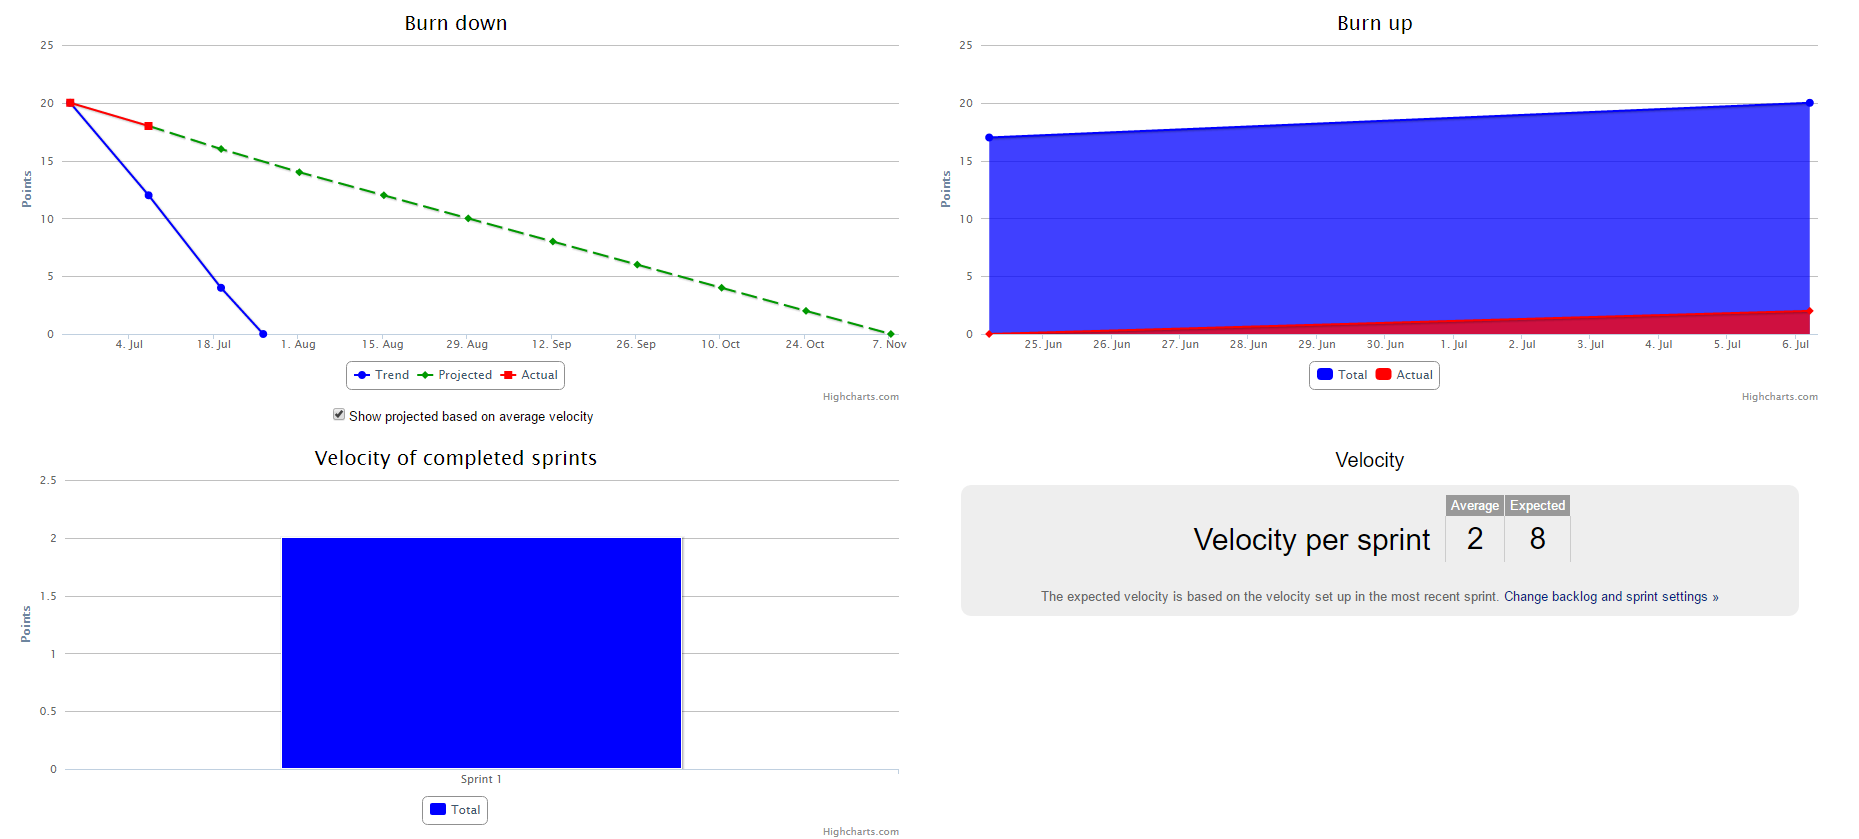
\includegraphics[width=0.9\textwidth]{images/Burndown_Sprint1}
    \caption{Example sprint burndown chart}
\end{figure}

\subsection{Sprint Retrospective}

At the end of each sprint the team discusses all of the sprint goals from the previous sprint, analyzes progress, and determines items that need to be changed or adjusted.

\subsection{Individual Status Reports}

Formal scrum meetings take place at the end of each class period with informal updates throughout the week via group messaging in GroupMe and emails/texting. 

\subsection{Engineering Notebooks}

Each individual team member is in charge of maintaining their own notebook, but ask for other team members to review as needed.

\subsection{Closeout Materials}

We will deliver the system as described in the mission statement and system overview to the University. The university will keep the Intel SR300 used by the project, and receive all related software, source code, and documentation in the form of a zip file. In addition, links will be provided to the online resources as described below. Other artifacts (Posters, supplemental materials, etc...) will also be provided to the university.

\subsubsection{System Prototype}

The system prototype will consist of open source software and an Intel SR300 camera. The university will retain the camera and software, with source code and documentation provided.

\subsubsection{Project Poster}

The team will collaborate to complete the poster and the end of Senior Design II.

\subsubsection{Source Code}

The source code will be maintained on GitHub, with each team member having access. The repository will be made public and the project will be made available as open source code for others to use and change.

\subsubsection{Source Code Documentation}

The source code documentation will be maintained with the source code in GitHub.

\subsubsection{Installation Scripts}

Instillation scripts will be maintained with the source code in GitHub.

\subsubsection{User Manual}

The user manual will help describe the use of the system to a user. It will be designed by the team and maintained in GitHub with the source code.
\newpage

%%% References
\bibliographystyle{plain}
\bibliographystyle{reference/IEEEtran_custom}
\bibliography{reference/refs}{}

\end{document}